

\begin{frame}[ctb!]
  \frametitle{Radionuclide Transport}
  % Map the path out of the repository.
  % WP failure, WF dissolution, 
  \begin{minipage}{0.49\textwidth}
  \begin{figure}[h!]
      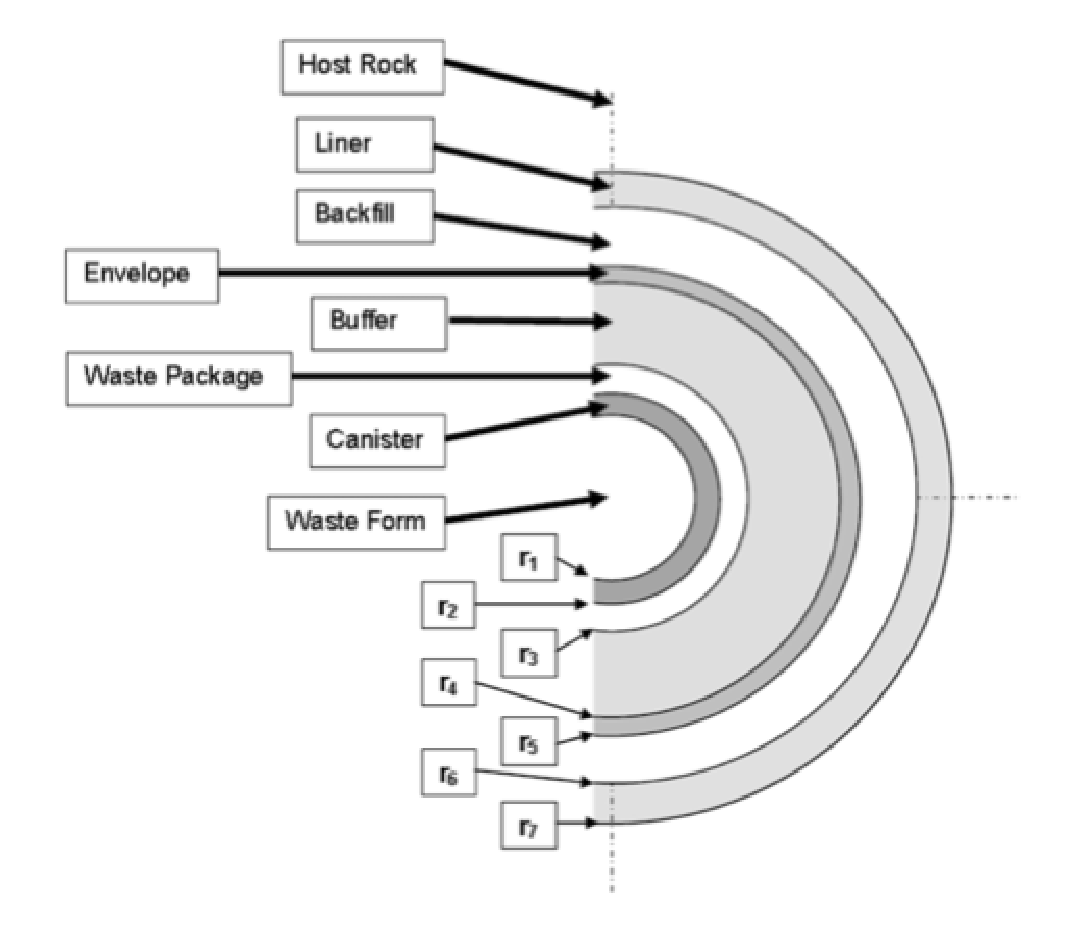
\includegraphics[width=\textwidth]{ebsLayersLLNL.eps}
    \caption{After waste package failure, radionuclides pass through successive 
    layers of the engineered barrier system \cite{greenberg_thermal_2011}.}
    \label{fig:ebsLayersLLNL}
  \end{figure}
  \end{minipage}
  \hspace{0.01cm}
  \begin{minipage}{0.49\textwidth}
    \begin{itemize}
      \item Source Term - Radionuclide mass flux to the environment
        \begin{itemize}
          \item Safety and Risk Metric
          \item EPA Regulation
        \end{itemize}
      \item Radionuclide transport is a function of
        \begin{itemize}
          \item Geochemistry - chemically induced material degradation, 
            radionuclide solubility limits, sorption, colloid mobility, etc.
          \item Hydrology - water induced material degradation, 
            water movement through pores and fractures, 
            dissolved contaminant dispersion. 
          \item Thermal Effects - thermally induced material degradation, 
            thermal hydrological effects.
        \end{itemize}
    \end{itemize}
  \end{minipage}
\end{frame}


\begin{frame}[ctb!]
  \frametitle{Waste Form Release Models}
  % Waste forms
  \footnotesize{%        File: litrev/wf_tab.tex
%     Created: Fri Aug 05 09:00 AM 2011 C
% Last Change: Fri Aug 05 09:00 AM 2011 C
%
\begin{table}[h!]
  \centering
  \footnotesize{
  \begin{tabular}{|l|l|c|c|}
    \multicolumn{4}{c}{\textbf{Waste Form Types}}\\
    \hline
    WF Type & SubTypes & Contents & Release Drivers  \\
    \hline
    \hline
    Once Through & \gls{CSNF} Ceramic Oxide & Nominal Burnup UOx \& MOX & redox reactions \\
                 & \gls{CSNF} Ceramic Oxide & High Burnup  & redox reactions, heat  \\
                 & \gls{HTGR} TRISO Graphite & High Burnup & graphite reactions\\
                 & \gls{DSNF} Metal  & High Burnup N Reactor Fuel & metal reactions,  heat\\
                 & \gls{DSNF} Carbides  & Fast Reactor Fuels & carbide reactions,  heat\\
                 & \gls{DSNF} Ceramic Oxides  & Research Reactor Fuels & redox reactions,  heat\\
    \hline
    Borosilicate Glass & Current & \glspl{MA} Cs/Sr & heat, glass alteration \\
                       & Future & Mo, no \gls{MA} no Cs/Sr & glass alteration  \\
    \hline
    Glass Ceramic & Glass Bonded Sodalite & Echem processed oxide fuels & ceramic, redox, glass reactions  \\
    \hline
    Metal Alloy & From Echem & Cladding, noble metals & metal reactions, heat \\
                & From Aqueous & undissolved solids, transition metals & metal reactions, heat  \\
    \hline
    Advance Ceramic &  & volatized iodine  & ceramic reactions, redox \\
    \hline
    Salt  & Cementitious Sodium  & separated streams  & alkaline reactions, dissolution \\
    \hline
  \end{tabular}
  \caption[Waste Form Types]{An array of waste forms developed for nuclear 
  wastes will have an array of dominant release 
  mechanisms.\cite{blink_disposal_2010}}
  \label{tab:wf}
  }
\end{table}


}
\end{frame}


\begin{frame}[ctb!]
  \frametitle{Waste Package Failure Models}
  % Waste Package
   
    \footnotesize{
    Waste package failure can, in general, be represented with an expression of the 
    number of failed waste packages, $n_F$ failing per unit time. This is a simple 
    product between the initial number of waste packages, $N$, and the rate, $f$, of 
    failure,
    \begin{align}
      n_F = N\cdot f().
      \intertext{This rate may be a physical function,}
      f() = N\cdot f(t,T,\cdots).
      \intertext{or any time dependent function,}
      f()=f(t).
      \intertext{of which instantaneous failure is a special case,}
      f()= \delta(t-t_F).
      \intertext{as is the Weibull distribution,}
      f(t,\lambda,k) =  \begin{cases}
        \frac{k}{\lambda}\left(\frac{t}{\lambda}\right)^{k-1}e^{-(t/\lambda)^{k}} & 
        t\geq0 ,\\
        0 & t<0 .\end{cases}
    \end{align}
    }
\end{frame}

\begin{frame}[ctb!]
  \frametitle{Waste Package Failure Models}
  % Waste Package
  \footnotesize{
  \begin{table}[h!]
\centering
\footnotesize{
\begin{tabular}[h!bt]{|l|r|r|r|}
  \multicolumn{4}{c}{\textbf{Current Waste Package Failure Models}}\\
  \hline
  Model&WP Failure Mode&Waste Form&Details\\
  \hline
  TSPA&EBSFAIL&&$300,000$ years\\
  \hline
  Ahn 2003&Instantaneous Failure&Borosilicate Glass&$t=0$\\
  \hline
  Ahn 2007& &CSNF $UO_2$ matrix &$T_f=75,000$ years\\
  & &Borosilicate Glass &$T_f=75,000$ years\\
  & & Naval $UO_2$ matrix &$T_f=75,000$ years\\
  \hline
  Li&EBSFAIL&&$300,000$ years\\
  \hline
  Hedin 2003& Instantaneous & Copper KBS-3 Concept & $t_{delay} = 300$ years \\
  \hline
\end{tabular}
\label{tab:wpfail}
\caption[Current WP Failure Models]{The above represent current methods by which waste packeage 
failure rates are modeled.}
}
\end{table}

  }
\end{frame}


\begin{frame}[ctb!]
  \frametitle{Solute Transport in Permeable Porous Media}
\begin{align} 
  \frac{\partial n C}{\partial t} & = - \nabla \cdot  (F_c + F_{dc} + F_d) + m 
  \label{solperm}
\end{align}
  \begin{minipage}{.49\textwidth}
    \footnotesize{
    \begin{align}
      \intertext{where} 
      \displaybreak[0]
      n &= \mbox{solute accessible porosity } [\%]\nonumber\\
      C &= \mbox{ concentration } [kg \cdot m^{-3}]\nonumber\\ 
      t &= \mbox{ time } [s]\nonumber\\ 
      F_c &= \mbox{ advective transport} [kg \cdot m^{-2}\cdot s^{-1}]\nonumber\\
      &= nvC \nonumber \\
      \displaybreak[0]
      F_{dc} &= \mbox{ dispersive transport} [kg \cdot m^{-2}\cdot s^{-1}]\nonumber\\ 
      &= \alpha nv \nabla C  \nonumber\\ 
      F_d &= \mbox{ diffusive transport} [kg \cdot m^{-2}\cdot s^{-1}]\nonumber\\
      &= D_e \nabla C\nonumber
    \end{align}}
  \end{minipage}
  \hspace{0.01cm}
  \begin{minipage}{.49\textwidth}
    \footnotesize{
    \begin{align}
      m &= \mbox{ solute source } [kg \cdot m^{-3}\cdot s^{-1}].\nonumber\\
      v &= \mbox{ pore velocity } [m\cdot s^{-1}] \nonumber\\
      \alpha &= \mbox{ dispersivity } [m]\nonumber\\
      D_e &= \mbox{ effective diffusion coefficient } [m^2\cdot s^{-1}]\nonumber
      \intertext{and} 
      n\cdot v &= \mbox{ Darcy velocity } [m\cdot s^{-1}].
    \end{align} }
  \end{minipage}
\end{frame}


\begin{frame}[ctb!]
  % Dispersion
\frametitle{Dispersion}
It is customary to define the combination of molecular diffusion, $D_e$ and mechanical dispersion, $\alpha v$, as $D$ 
\begin{align}
  D = \alpha v + D_e
\end{align}
such that the mass conservation equation becomes:
\begin{align}
  \frac{\partial(nC)}{\partial t} &= \nabla \left( nD\nabla C \right) - \nabla \left( nvC \right) 
  \label{massbal} 
  \intertext{Adding sorption, by accounting for a change in mass storage,}
  \frac{\partial(nC)}{\partial t}  + \frac{\partial(s\rho_b)}{\partial t} &= 
  \nabla \left( nD\nabla C \right) - \nabla \left( nvC \right)  
  \label{withsorption} 
  \intertext{where}
  s &= \mbox{sorption coefficient}\nonumber\\
  \rho_b &= \mbox{ bulk (dry) density }[kg/m^3].\nonumber
\end{align}
\end{frame}



\begin{frame}[ctb!]
  \frametitle{Dimensionality}
  \begin{figure}[h!]
    \begin{center}
      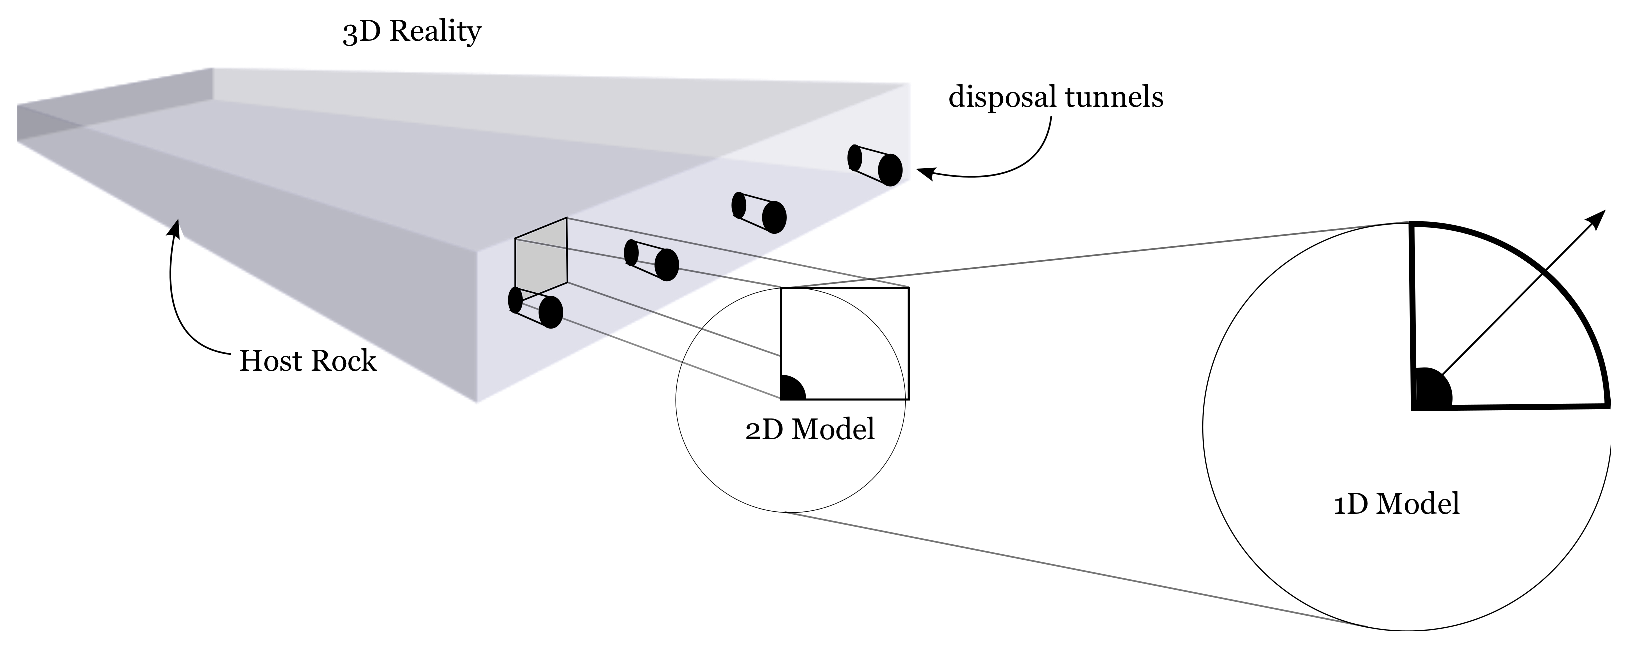
\includegraphics[width=0.9\textwidth]{3dto1d.eps}
    \end{center}
    \caption{Employing the symmetries of the disposal layout can enable lower 
    dimensional models.}
    \label{fig:3dto1d}
  \end{figure}
\end{frame}

\begin{frame}[ctb!]
  \frametitle{Dispersion}
For unidirectional flow, the unidirectional dispersion tensor gives 
\begin{align}
  D_x \frac{\partial^2 C}{\partial x^2} +
  D_y \frac{\partial^2 C}{\partial y^2} +
  D_z \frac{\partial^2 C}{\partial z^2} +
  v_x \frac{\partial C}{\partial x}  = R_f 
  \frac{\partial(nC)}{\partial t}. 
  \label{unidirflow}
\end{align}
\end{frame}

\begin{frame}[ctb!]
  \frametitle{Diffusion}
A special case of uniform flow, no flow, simplifies to the diffusion equation,
\begin{align}
  D_x \frac{\partial^2 C}{\partial x^2} +
  D_y \frac{\partial^2 C}{\partial y^2} +
  D_z \frac{\partial^2 C}{\partial z^2} +
  = R_f 
  \frac{\partial(nC)}{\partial t} .
  \label{diffusion}
\end{align}
\end{frame}

\begin{frame}[ctb!]
  % Precipitation
  \frametitle{Precipitation}
  Elemental solubility limits are based on the maximum concentration of an 
  element which can exist in solution.

    \begin{align} 
      m_{1i}(t)\le v_{1i}(t)C_{sol}
      \intertext{where}
      m_{li} = \mbox{dissolved kg of radionuclide i}\nonumber\\
      v_{li} = \mbox{void volume}\nonumber\\
      C_{sol} = \mbox{solubility limit}\nonumber
    \end{align}
    
\end{frame}

\begin{frame}[ctb!]
  \frametitle{Sorption}
  % Sorption
If it is assumed that sorption can be approximated as a linear equilibrium, 
reversible reaction,
\begin{align}
  \frac{\partial(s\rho_b)}{\partial t} &= \left( R_f - 1 
  \right)\frac{\partial(nC)}{\partial t}
  \intertext{equation \eqref{withsorption} becomes}
  \nabla \left( nD\nabla C \right) - \nabla \left( nv \right) &= 
  R_f\frac{\partial(nC)}{\partial t}   
  \label{withlinsorption}
  \intertext{where}
  R_f &= \mbox{retardation factor}\nonumber\\
  &= 1+\frac{\rho_bK_d}{n}\\
  \rho_b &=\mbox{bulk density of the rock matrix}\nonumber
  \intertext{and}
  K_d &= \mbox{species distribution coefficient.}\nonumber
\end{align}
\end{frame}




  % Ogata and Banks
\begin{frame}[ctb!]
  \frametitle{One Dimensional Solution with a Constant Concentration Source}
An analytical solution for the one dimensional case with a continuous source 
of constant concentration is known \cite{schwartz_fundamentals_2004}. For the boundary conditions
\begin{align}
  C(0,t) =& C_0
  \intertext{and}
  \frac{\partial C}{\partial x}\Big|_{x=\infty} =& 0
  \label{BCs}
  \intertext{as well as the initial condition }
  C(x,0) =& 0 \mbox{\hspace{2mm}for\hspace{1mm}} x \in (0,\infty),
\end{align}
the Ogata and Banks solution gives
\begin{align}
  C(x,t) =& \frac{C_0}{2}\left[
  \erfc{\left( \frac{x- \frac{v_x t}{R_f} }{2\sqrt{ 
  \frac{D_xt}{R_f} }} \right)} +
  e^{\frac{v_xx}{D_x}}
  \erfc{\left( \frac{x+ \frac{v_x t}{R_f} }{2\sqrt{ 
  \frac{D_xt}{R_f} }} \right)}
  \right].
  \label{ogatabanks}
  \intertext{where}
  \erfc(x) =& \frac{2}{\sqrt{\pi}}\int_x^\infty e^{-t^2}dt. 
\end{align}
\end{frame}


